\begin{figure}[!htb]
    \centering
    \begin{subfigure}[b]{0.49\textwidth}
        \centering
        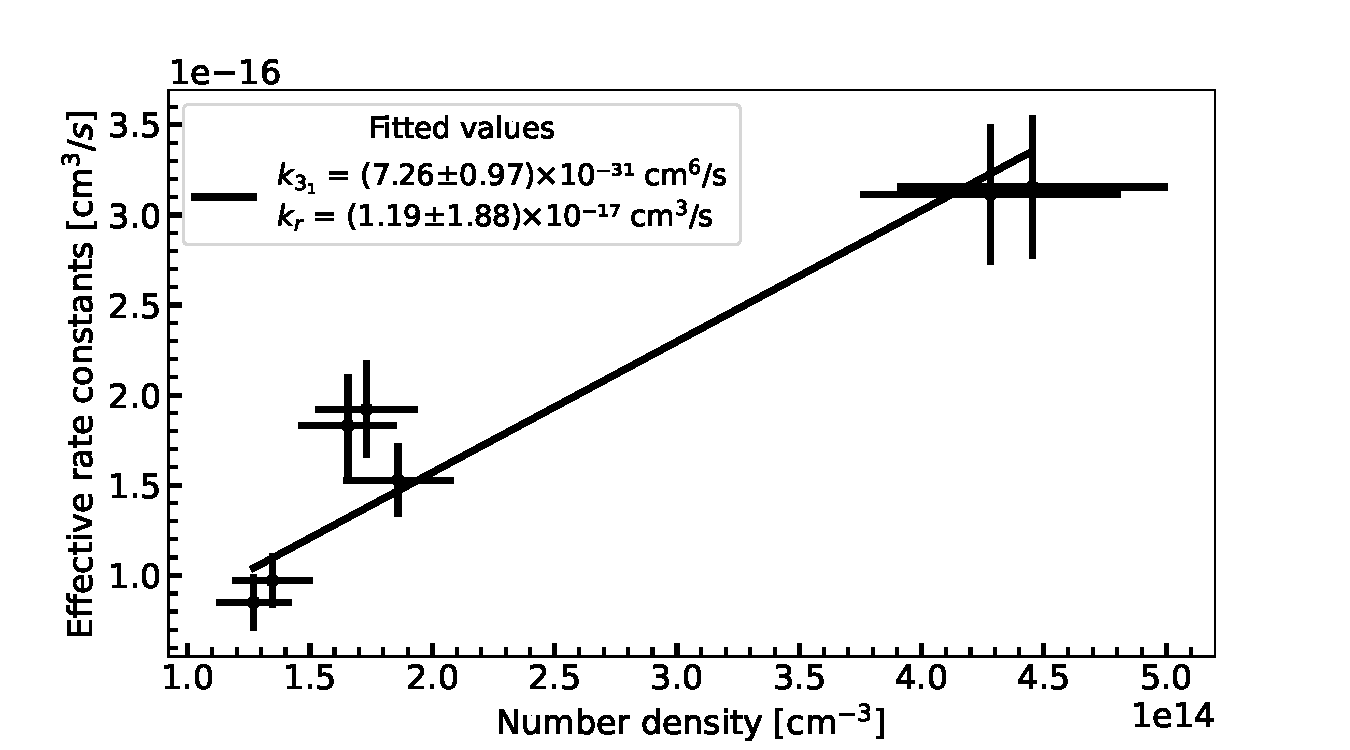
\includegraphics[width=1\textwidth]{figures/measurements/kinetics/functionOf_nHe/on_4.8K_k31_effective_rate_constants.pdf}
        \caption{}
        \label{fig:on:effective-rate-constants}
    \end{subfigure}
    \hfill
    \begin{subfigure}[b]{0.49\textwidth}
        \centering
        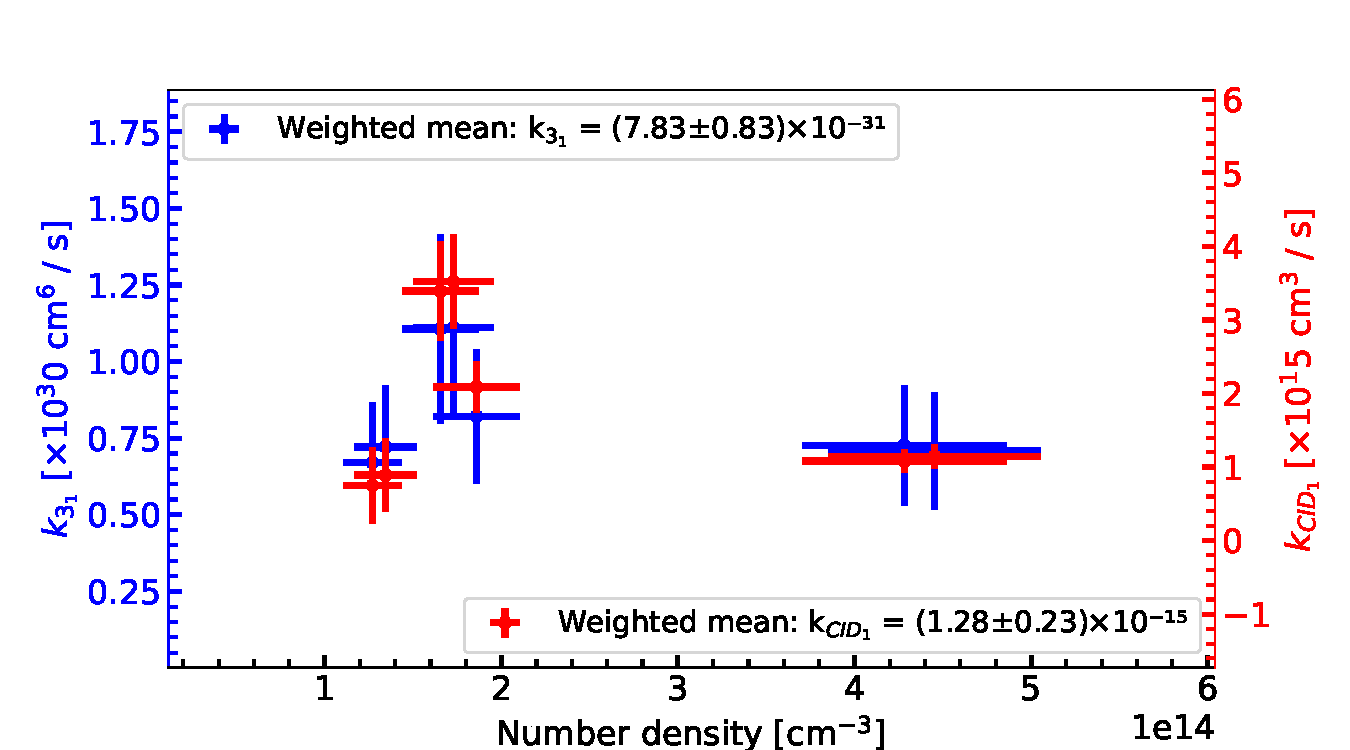
\includegraphics[width=1\textwidth]{figures/measurements/kinetics/functionOf_nHe/on_4.8K_k3_kCID_1_as_functionOfnHe.pdf}
        \caption{}
        \label{fig:on:rate-constants}
    \end{subfigure}

    \caption{Deriving rate coefficients in the presence of radiation resonant with the $J=0-1$ transition of \CD. (a) The effective binary rate constant ($k_e$) is plotted as a function of number density to derive $k_{3_1}$ (ternary association) and $k_r$ (radiative) rate constants. The solid line indicates the linear fit where the slope and intercept correspond to $k_3$ and $k_r$, respectively. (b) shows the ternary association (\textcolor{blue}{$k_{3_1}$}) and collision-induced dissociation (\textcolor{red}{$k_{CID_1}$}) rate constants plotted as a function of helium number density under the assumption: $k_3[He] \gg k_r$(see text). The weighted mean values are shown in the legend box.}
    \label{fig:on:effective-and-ternary}

\end{figure}
